\documentclass[letterpaper,12pt]{article}

\usepackage{tabularx} % extra features for tabular environment
\usepackage{amsmath}  % improve math presentation
\usepackage{graphicx} % takes care of graphic including machinery
\usepackage[margin=1in,letterpaper]{geometry} % decreases margins
\usepackage{cite} % takes care of citations
\usepackage[final]{hyperref} % adds hyper links inside the generated pdf file
\usepackage{ctex}
\usepackage{titlesec}
%\usepackage{CJKutf8, CJK}
\usepackage{makecell}                 % 三线表-竖线
\usepackage{booktabs}                 % 三线表-短细横线
% \usepackage{natbib}
\usepackage{graphicx}				  % 表格单元格逆时针
\usepackage{multirow}				  % 合并单元格
\usepackage{array}
\usepackage{amssymb}				  % 勾
\usepackage{amsmath}
\usepackage{longtable}                % 导入 longtable 宏包,表格自动换行
\usepackage{caption}
\usepackage{subcaption}               % 设置子图
\usepackage{color}					  % 文本颜色包
\usepackage{xcolor}
\usepackage{bbm}					  % 输入指示函数
\usepackage{tablefootnote}			  % 表格注释
\usepackage{pythonhighlight}

\usepackage{listings}                 % 导入代码块
\usepackage{xcolor}
\lstset{
	numbers=left, 
	tabsize=1,
	columns=flexible, 
	numberstyle=  \small, 
	keywordstyle= \color{ blue!70},
	commentstyle= \color{red!50!green!50!blue!50}, 
	frame=shadowbox, % 阴影效果
	rulesepcolor= \color{ red!20!green!20!blue!20} ,
	escapeinside=``, % 英文分号中可写入中文
	xleftmargin=2em,
	xrightmargin=2em, 
	aboveskip=1em,
} 

\hypersetup{
	colorlinks=true,       % false: boxed links; true: colored links
	linkcolor=blue,        % color of internal links
	citecolor=blue,        % color of links to bibliography
	filecolor=magenta,     % color of file links
	urlcolor=blue         
}
%++++++++++++++++++++++++++++++++++++++++
\titleformat{\section}{\Large\bfseries\songti}{\thesection}{1em}{}
\titleformat{\subsection}{\large\bfseries\songti}{\thesubsection}{1em}{}
\titleformat{\subsubsection}{\normalsize\bfseries\songti}{\thesubsubsection}{1em}{}
\titleformat{\paragraph}{\small\bfseries\songti}{\paragraph}{1em}{}
\titleformat{\subparagraph}{\footnotesize\bfseries\songti}{\subparagraph}{1em}{}

\begin{document}
	
	
	\title{\songti \zihao{4}5月21日-5月29日工作汇报}
	\author{\textrm{Ku Jui}}
	\date{\textrm{May 2023}}
	\maketitle
	
	\renewcommand{\figurename}{Figure} % 可以重新定义abstract,因为ctex会覆盖thebibliography
	% 	\begin{abstract}
		%		In this experiment we studied a very important physical effect by measuring the
		%		dependence of a quantity $V$ of the quantity $X$ for two different sample
		%		temperatures.  Our experimental measurements confirmed the quadratic dependence
		%		$V = kX^2$ predicted by Someone's first law. The value of the mystery parameter
		%		$k = 15.4\pm 0.5$~s was extracted from the fit. This value is
		%		not consistent with the theoretically predicted $k_{theory}=17.34$~s. We attribute %this
		%		discrepancy to low efficiency of our $V$-detector.
		%	\end{abstract}
	\renewcommand{\contentsname}{Contents}
	
	\tableofcontents  % 自动生成目录
	
	\section{文献阅读}
	
	\subsection{Pre-knowledge}
	
	模型中的损失函数是用来衡量模型的预测值和真实值(Ground Truth)之间的差异程度的函数,它可以反映模型的优化方向和性能指标\footnote{https://zhuanlan.zhihu.com/p/375968083}。它是一种衡量模型预测结果与真实结果之间差异的方法,用于指导模型参数的更新。在训练过程中,通过不断最小化损失函数来优化模型参数,使模型能够更好地拟合数据\footnote{https://zhuanlan.zhihu.com/p/436809988}。因此,需要使用合适的损失函数,当模型在数据集上进行训练时,该函数可以适当地惩罚模型 \footnote{https://zhuanlan.zhihu.com/p/473113939}。
	
	不同的损失函数适用于不同的任务和数据分布,例如回归问题常用的有均方误差损失函数(MSE,也叫做$\mathcal{L}_{2}$损失函数)和$\mathcal{L}_{1}$损失函数,分类问题常用的有交叉熵损失函数(Cross Entropy Loss)等\footnote{https://blog.csdn.net/weixin\_57643648/article/details/122704657}。损失函数的选择会影响模型的收敛速度和精度,因此需要根据具体情况选择合适的损失函数\footnote{https://www.zhihu.com/tardis/zm/art/136047113?source\_id=1005}。
	
	目前常用的损失函数是从相关视觉任务中借用的,但这些损失函数可能并不完全适用于低照度图像增强LLIE。因此,需要设计更适合 LLIE 的损失函数,以更好地驱动深度网络的优化。这可以通过研究人类对图像质量的视觉感知来实现,使用深度神经网络来近似人类视觉感知,并将这些理论应用于损失函数的设计。损失函数可以分为两个大类:回归问题和分类问题。
	
	
	
	\subsubsection{loss function for CV}
	
	\paragraph{$\mathcal{L}_1$-loss}
	
	平均绝对误差(MAE)损失,也称$\mathcal{L}_1$范数损失,计算实际值和预测值之间绝对差之和的平均值。
	
	\begin{equation}
		\begin{aligned}
			\mathcal{L}_1 = \frac{1}{N} \sum_{i=1}^{N} {\| \hat{y}_i - y_i \|}_{1}
		\end{aligned}
	\end{equation}
	
	适用于回归问题,MAE loss对异常值更具鲁棒性,尤其是当目标变量的分布有离群值时(小值或大值与平均值相差很大)。
	
	函数:\textit{torch.nn.L1Loss}
	
	\paragraph{$\mathcal{L}_2$-loss}
	
	均方误差(MSE)损失,也称为$\mathcal{L}_2$范数损失,计算实际值和预测值之间平方差的平均值\footnote{https://blog.csdn.net/yanyuxiangtoday/article/details/119788949}。
	
	\begin{equation}
		\begin{aligned}
			\mathcal{L}_1 = \frac{1}{N} \sum_{i=1}^{N} {\| \hat{y}_i - y_i \|}_{2}^2
		\end{aligned}
	\end{equation}
	
	
	平方意味着较大的误差比较小的误差会产生更大的惩罚,所以$\mathcal{L}_2-loss$的收敛速度要比$\mathcal{L}_1-loss$要快得多。但是,$\mathcal{L}_2-loss$对异常点更敏感,鲁棒性差于$\mathcal{L}_1-loss$。
	
	$\mathcal{L}_1-loss$损失函数相比于$\mathcal{L}_2-loss$损失函数的鲁棒性更好。因为以$\mathcal{L}_2-loss$范数将误差平方化(如果误差大于1,则误差会放大很多),模型的误差会比以$\mathcal{L}_1-loss$范数大的多,因此模型会对这种类型的样本更加敏感,这就需要调整模型来最小化误差。但是很大可能这种类型的样本是一个异常值,模型就需要调整以适应这种异常值,那么就导致训练模型的方向偏离目标了\footnote{https://zhuanlan.zhihu.com/p/137073968}。
	
	对于大多数回归问题,一般是使用$\mathcal{L}_2-loss$而不是$\mathcal{L}_1-loss$。
	
	函数: \textit{torch.nn.MSELoss}
	
	\paragraph{Regularization of the $\mathcal{L}_1$ and $\mathcal{L}_2$ loss functions}
	
	正则化的基本思想是通过在损失函数中加入额外信息,以便防止过拟合和提高模型泛化性能。无论哪一种正则化方式,基本思想都是希望通过限制权重的大小,使得模型不能任意拟合训练数据中的随机噪声,正则化实际是在损失函数中加入刻画模型复杂程度的指标\footnote{https://blog.csdn.net/weixin\_41960890/article/details/104891561}。
	
	对应的L1正则损失函数:
	
	\begin{equation}
		\begin{aligned}
			\mathcal{L}_{norm1} = \mathcal{L}_{1}{\left(\hat{y},y\right)} + \lambda \sum_{\omega}{\| \omega \|}_1
		\end{aligned}
	\end{equation}
	
	对应的L2正则损失函数:
	
	\begin{equation}
		\begin{aligned}
			\mathcal{L}_{norm2} = \mathcal{L}_{2}{\left(\hat{y},y\right)} + \lambda \sum_{\omega}{\| \omega \|}^2_2
		\end{aligned}
	\end{equation}
	
	假设$\mathcal{L}_{1}{\left(\hat{y},y\right)}$和$\mathcal{L}_{2}{\left(\hat{y},y\right)}$是未加正则项的损失,$\lambda$是一个超参,用于控制正则化项的大小,惩罚项$\omega$用于惩罚大的权重,隐式地减少自由参数的数量。
	
	正则化是如何降低过拟合现象的?
	
	正则化之所以能够降低过拟合的原因在于,正则化是结构风险最小化的一种策略实现。给损失函数加上正则化项,能使得新得到的优化目标函数$h = f + normal$ ,需要在$f$和$normal$中做一个权衡(trade-off),如果还像原来只优化$f$的情况下,那可能得到一组解比较复杂,使得正则项$normal$比较大,那么$h$就不是最优的,因此可以看出加正则项能让解更加简单,符合奥卡姆剃刀理论,同时也比较符合在偏差和方差(方差表示模型的复杂度)分析中,通过降低模型复杂度,得到更小的泛化误差,降低过拟合程度\footnote{https://zhuanlan.zhihu.com/p/35356992}。
	
	PyTorch实现: $\mathcal{L}_2$正则项是通过optimizer优化器的参数 weight\_decay(float, optional) 添加的,用于设置权值衰减率,即正则化中的超参$\lambda$,默认值为0。
	
	\lstset{language=python,breaklines=true}
	\begin{lstlisting}
		optimizer = torch.optim.SGD(model.parameters(),lr=0.01,weight_decay=0.01)
	\end{lstlisting}
	
	\paragraph{Smooth $\mathcal{L}_1$ loss function}
	
	Smooth $\mathcal{L}_1$损失函数是由Girshick R在Fast R-CNN中提出的,主要用在目标检测中防止梯度爆炸。它是一个分段函数,在$\left[-1,1\right]$之间是$\mathcal{L}_2$损失,其他区间就是$\mathcal{L}_1$损失。这样即解决了$\mathcal{L}_1$损失在0处不可导的问题,也解决了$\mathcal{L}_2$损失在异常点处梯度爆炸的问题\footnote{https://zhuanlan.zhihu.com/p/261059231}。
	
	\begin{equation}
		\text{smooth} \ \mathcal{L}_1 \ \text{loss} = \frac{1}{N}\sum_{i=1}^{N}
		\left\{
		\begin{aligned}
			&\frac{{\|\hat{y}_i - y_i \|}_2^{2}}{2\beta}, \| \hat{y}_i -y_i \| < \beta , \\
			&{\|\hat{y}_i - y_i \|}_1 - \frac{1}{2}\beta, \| \hat{y}_i -y_i \| \geq \beta.
		\end{aligned}
		\right.
	\end{equation}		
	
	一般取$\beta=1$。smooth $\mathcal{L}_1$和$\mathcal{L}_1$-loss函数的区别在于, smooth $\mathcal{L}_1$在0点附近使用$\mathcal{L}_2$使得它更加平滑, 它同时拥有$\mathcal{L}_2$-loss和$\mathcal{L}_1$-loss的部分优点。
	
	函数:\textit{torch.nn.SmoothL1Loss}
	
	\paragraph{Huber loss function}
	
	$\mathcal{L}_2$-loss但容易受离群点的影响,$\mathcal{L}_1$-loss对离群点更加健壮但是收敛慢,Huber Loss 则是一种将MSE与MAE结合起来,取两者优点的损失函数,也被称作Smooth Mean Absolute Error Loss。其原理很简单,就是在误差接近0时使用$\mathcal{L}_2$-loss,误差较大时使用$\mathcal{L}_1$-loss
	
	\begin{equation}
		J_{Huber}(\delta)= \frac{1}{N}\sum_{i=1}^{N}
		\left\{
		\begin{aligned}
			&\frac{1}{2}{\left\|\hat{y}_i - y_i \right\|}_2^{2}, \left\| \hat{y}_i -y_i \right\| < \delta , \\
			&\delta\left({\left\|\hat{y}_i - y_i \right\|}_1 - \frac{1}{2}\delta \right), \left\| \hat{y}_i -y_i \right\| \geq \delta.
		\end{aligned}
		\right.
	\end{equation}
	
	残差比较小时,Huber Loss是二次函数;残差比较大时,Huber Loss是线性函数(残差,即观测值和预测值之间的差值)。与$\mathcal{L}_2$-loss相比,Huber损失对数据中的异常值不那么敏感。使函数二次化的小误差值是多少取决于“超参数”$\delta$,它可以调整。当$\delta=1$时,退化成smooth $\mathcal{L}_1$ Loss。
	
	函数:\textit{torch.nn.HuberLoss}
	
	\paragraph{log-MSE}
	
	\begin{equation}
		\begin{aligned}
			J_{log-MSE} = 10\log_{10}\left(\frac{1}{N} \sum_{i=1}^{N} {\| \hat{y}_i - y_i \|}_{2}^2 \right)
		\end{aligned}
	\end{equation}
	
	\paragraph{Perceptual loss function}
	
	感知损失(Perceptual Loss)是一种用于比较两个看起来相似的图像的损失函数,这一损失函数由Johnson et al.\cite{johnson2016perceptual}提出。它用于比较图像之间的高层次差异,如内容和风格差异\footnote{https://deepai.org/machine-learning-glossary-and-terms/perceptual-loss-function}。它已被广泛用作图像合成任务(包括图像超分辨率和风格转换)中的有效损失项。
	
	感知损失函数用于比较两个看起来相似的不同图像,例如同一张照片,但偏移了一个像素。该函数用于比较图像之间的高级差异,例如内容和样式差异。感知损失函数与每像素损失函数非常相似,因为两者都用于训练前馈神经网络以进行图像转换任务。感知损失函数是一个更常用的组件,因为它通常提供有关风格迁移的更准确的结果。
	
	简而言之,感知损失函数的工作原理是将所有像素之间的所有平方误差相加并取平均值。这与每像素损失函数形成对比,后者对像素之间的所有绝对误差求和\cite{johnson2016perceptual}。
	
	作者认为感知损失函数不仅在生成高质量图像方面更准确,而且在优化后也快了三倍。神经网络模型在图像上进行训练,其中感知损失函数基于从已训练网络中提取的高级特征进行优化。
	
	\begin{equation}
		\begin{aligned}
			\ell_{feat}^{\phi,j} (\hat{y},y) = \frac{1}{C_{j}H_{j}W_{j}}{\left\| \phi_{j}(\hat{y})-\phi_{j}(y)\right\|}_{2}^2
		\end{aligned}
		\label{eq: perceptual loss}
	\end{equation}
	
	其中$\hat{y}$为输出图像,$y$为目标图像,$\phi$为损失网络。$\phi_{j}(x)$为处理图像$x$时损失网络$\phi$的第$j$层的激活情况,如果$j$是一个卷积层,那么$\phi_{j}(x)$将是形状$C_{j} \times H_{j} \times W_{j}$的特征映射,特征重建损失是特征表示之间的欧式距离,如eq \ref{eq: perceptual loss}。
	
	\begin{figure}[ht] 
		% read manual to see what [ht] means and for other possible options
		\centering 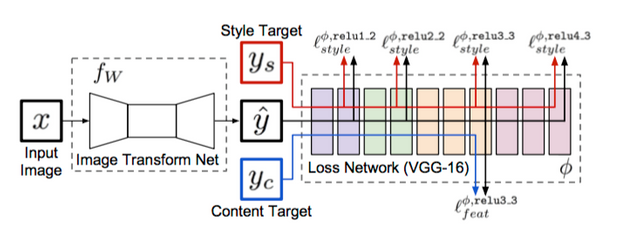
\includegraphics[width=0.8\columnwidth]{perceptual}
		\captionsetup{font=scriptsize}
		\caption{
			\label{fig: perceptual loss} % spaces are big no-no withing labels
			% things like fig: are optional in the label but it helps
			% to orient yourself when you have multiple figures,
			% equations and tables
			System overview. We train an image transformation network to transform input images into output images. We use a loss network pretrained for image classification to define perceptual loss functions that measure perceptual differences in content and style between images. The loss network remains fixed during the training process.
		}
	\end{figure}
	
	Fig.\ref{fig: perceptual loss}表示经过训练以将输入图像转换为输出图像的神经网络。用于图像分类的预训练损失网络有助于通知损失函数。预先训练的网络有助于定义测量图像之间内容和风格的感知差异所需的感知损失函数。
	
	对于图像数据来说,网络在提取特征的过程中,较浅层通常提取边缘、颜色、亮度等低频信息,而网络较深层则提取一些细节纹理等高频信息,再深一点的网络层则提取一些具有辨别性的关键特征,也就是说,网络层越深提取的特征越抽象越高级。
	
	感知损失就是通过一个固定的网络(通常使用预训练的VGG16或者VGG19),分别以真实图像(Ground Truth)、网络生成结果(Prediciton)作为其输入,得到对应的输出特征:feature\_gt、feature\_pre,然后使用feature\_gt与feature\_pre构造损失(通常为$\mathcal{L}_2$-loss),逼近真实图像与网络生成结果之间的深层信息,也就是感知信息,相比普通的$\mathcal{L}_2$-loss而言,可以增强输出特征的细节信息\footnote{https://blog.csdn.net/qq\_43665602/article/details/127077484}。
	
	\paragraph{SSIM loss function}
	
	SSIM损失函数是一种用于衡量两幅图像之间差距的损失函数。它考虑了亮度、对比度和结构指标,这就考虑了人类视觉感知,一般而言,SSIM得到的结果会比$\mathcal{L}_1$-loss,$\mathcal{L}_2$-loss的结果更有细节\footnote{https://blog.csdn.net/u013289254/article/details/99694412}。
	
	每个像素$p$的\text{SSIM}被定义为
	\begin{equation}
		\begin{aligned}
			\text{SSIM}(p) &= \frac{2\mu_{x}\mu_{y}+C_{1}}{\mu_{x}^2+\mu_{y}^2+C_{1}} \cdot \frac{2\sigma_{xy}+C_{2}}{\sigma_{x}^2+\sigma_{y}^{2}+C_{2}} \\
			&= l(p)\cdot cs(p)
		\end{aligned}
		\label{eq: SSIM}
	\end{equation}
	其中省略了均值和标准偏差对像素$p$的依赖性,均值和标准差是用标准偏差为$\sigma_G,G_{\sigma_G}$
	\begin{equation}
		\begin{aligned}
			&\varepsilon(p)=1-\text{SSIM}(p): \\  &\mathcal{L}^{\text{SSIM}}(P)=\frac{1}{N}\sum_{p \in P}1-\text{SSIM}(p).
		\end{aligned}
		\label{eq: SSIM loss}
	\end{equation}
	
	eq. \ref{eq: SSIM}表明$\text{SSIM}(p)$需要关注像素$p$的邻域,这个领域的大小取决于$G_{\sigma_G}$,网络的卷积性质允许我们将SSIM损失写为
	
	\begin{equation}
		\begin{aligned}
			\mathcal{L}^{\text{SSIM}}(P)=1-\text{SSIM}(\tilde{p}).
		\end{aligned}
		\label{eq: revised_SSIM loss}
	\end{equation}
	
	其中$\tilde{p}$是$P$的中心像素。
	
	\paragraph{MS-SSIM loss function}
	
	多尺度结构相似性(MS-SSIM)损失函数是基于多层(图片按照一定规则,由大到小缩放)的SSIM损失函数,相当于考虑了分辨率\footnote{https://blog.csdn.net/u013289254/article/details/99694412}。它是一种更为复杂的SSIM损失函数,可以更好地衡量图像之间的相似性。
	
	\begin{equation}
		\begin{aligned}
			\text{MS-SSIM}(p)=l_{M}^\alpha(p)\cdot \prod_{j=1}^M cs_{j}^{\beta_j}(p)
		\end{aligned}
		\label{eq: MS-SSIM}
	\end{equation}
	
	其中$M,j$描述的是比例,设$\alpha=\beta_j=1$,对于$j={1,\cdots, M}$类似eq. \ref{eq: revised_SSIM loss},利用中心像素$\tilde{p}$处计算的损失来近似贴片$P$的损失:
	
	\begin{equation}
		\begin{aligned}
			\mathcal{L}^{\text{MS-SSIM}}(P)=1-\text{MS-SSIM}(\tilde{p})
		\end{aligned}
		\label{eq: MS-SSIM loss}
	\end{equation}
	
	\paragraph{Cross-entropy loss function}
	
	交叉熵损失函数是一种常用的分类问题损失函数。在二分类问题中,它的定义为Eq. \ref{eq: Cross-entropy loss}
	\begin{equation}
		\begin{aligned}
			\mathcal{L}(\hat{y},y)=-\left( y\log_{\hat{y}} + (1-y) \log (1-\hat{y}) \right)
		\end{aligned}
		\label{eq: Cross-entropy loss}
	\end{equation}
	
	其中,$\hat{y}$表示模型预测的概率值(即分类器输出),$y$表示样本真实的类别标签。对于正例样本($y=1$),交叉熵损失函数的值等于$log {\hat{y}}$;对于反例样本($y=0$),交叉熵损失函数的值等于$\log (1-\hat{y})$。 因此,交叉熵损失函数的目标是最小化模型预测与实际标签之间的差距,从而让模型能够更准确地进行分类。 
	
	交叉熵损失函数可以推广到多分类问题中,此时它的表达式略有不同。在多分类问题中,交叉熵损失函数可以写成以下形式: 
	\begin{equation}
		\begin{aligned}
			\mathcal{L}(\hat{y},y)=-\sum_{i=1}^K y_i \log \hat{y}_i
		\end{aligned}
		\label{eq: revised_Cross-entropy loss}
	\end{equation} 
	
	其中,$K$表示类别的数量,$y_i$表示第$i$个类别的真实标签,$\hat{y}_i$表示模型对于第$i$个类别的预测概率值。交叉熵损失函数的目标仍然是最小化预测与实际标签之间的差距,从而让模型能够更准确地进行分类。
	
	\paragraph{Adversarial loss function}
	
	Adversarial loss function是生成对抗网络(GAN)的标准损失函数。GAN是由生成器(Generator)和判别器(Discriminator)组成的两个神经网络模型。生成器的目标是生成与真实数据相似的假数据,而判别器的目标是将真实数据与生成的假数据区分开来。Adversarial loss使得GAN能够不断的改进生成器的性能,使其能够生成更加逼真的数据。
	
	\begin{figure}[htbp] 
		% read manual to see what [ht] means and for other possible options
		\centering 
		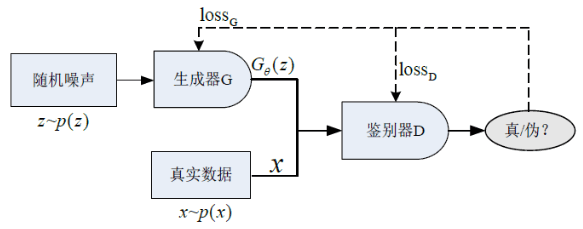
\includegraphics[width=0.8\columnwidth]{GAN_architecture}
		\captionsetup{font=scriptsize}
		\caption{
			\label{fig: GAN_architecture} % spaces are big no-no withing labels
			% things like fig: are optional in the label but it helps
			% to orient yourself when you have multiple figures,
			% equations and tables
			Computational flow and structure of the GAN.
		}
	\end{figure}
	
	如Fig. \ref{fig: GAN_architecture}所示,在训练过程中,生成器和判别器相互竞争和对抗。生成器试图生成逼真的假数据$G_\theta{\left( z \right)}$以欺骗判别器,而判别器则试图准确地判断真实数据和生成的假数据。Adversarial loss通过衡量生成器生成的假数据被判别器识别为真实数据的程度,来指导生成器的训练。它的目标是最小化生成器生成的假数据与真实数据之间的差异,使得判别器难以区分它们。
	
	一般而言,GAN的目标函数为$V(D, G)$Eq. \ref{eq: Adversarial loss}
	\begin{equation}
		\begin{aligned}
			\min_G \max_D V\left( D, G \right) = \mathbb{E}_{x \sim p_{data}(x)}\left[ \log D(x) \right] + \mathbb{E}_{z \sim p_{noise}(z)}\left[ \log \left(1- D(G(z))\right) \right]
		\end{aligned}
		\label{eq: Adversarial loss_another}
	\end{equation}
	
	其中,$E(*)$表示分布函数的期望值,$P_{data}(x)$代表着真实样本的分布,$P_{noise}(z)$是定义在低维的噪声分布,通过参数为$\theta_{g}$的$G$映射到高维的数据空间得到$P_g=G(z,\theta_{g})$,这些参数通过交替迭代的方法来进行优化,见Fig. \ref{fig: Alternate Optimization}。Fig. \ref{fig: D_optimization}固定$G$参数不变,优化$D$的参数,即最大化$\max V\left( D, G \right)$ 等价于$\min \left[ - V(D,G) \right]$。因此,$D$的损失函数等价于Eq. \ref{eq: Adversarial loss_another}
	\begin{equation}
		\begin{aligned}
			J^{D} \left( \theta^{D}, \theta^{G} \right) = -\mathbb{E}_{x \sim p_{data}(x)}\left[ \log D(x) \right] - \mathbb{E}_{\tilde{x} \sim p_{g}(x)}\left[ \log \left(1- D(\tilde{x})\right) \right]
		\end{aligned}
		\label{eq: Adversarial loss}
	\end{equation}
	
	\begin{figure}[htbp] 
		% read manual to see what [ht] means and for other possible options
		\centering 
		% 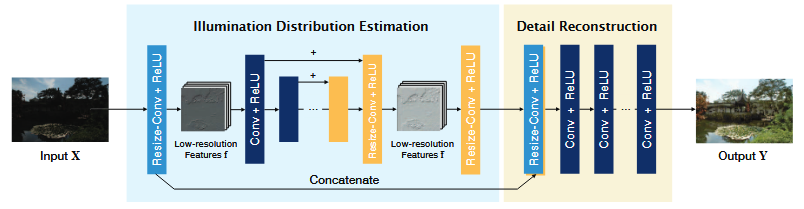
\includegraphics[width=0.8\columnwidth]{GLADNet}
		\begin{subfigure}{0.4\textwidth}
			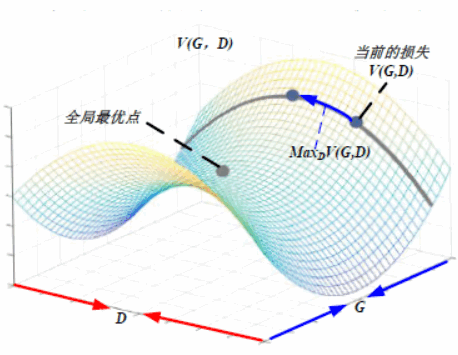
\includegraphics[width=\linewidth]{D_optimization}
			\captionsetup{font=scriptsize}
			\caption{D的优化过程}
			\label{fig: D_optimization}
		\end{subfigure}
		\begin{subfigure}{0.4\textwidth}
			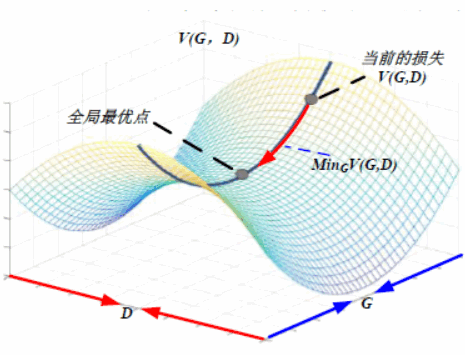
\includegraphics[width=\linewidth]{G_optimization}
			\captionsetup{font=scriptsize}
			\caption{G的优化过程}
			\label{fig: G_optimization}	
		\end{subfigure}
		\captionsetup{font=scriptsize}
		\caption{
			\label{fig: Alternate Optimization} % spaces are big no-no withing labels
			% things like fig: are optional in the label but it helps
			% to orient yourself when you have multiple figures,
			% equations and tables
			The optimization of the GAN parameters 
		}
	\end{figure}
	
	
	Adversarial loss的具体形式可以根据具体的GAN架构和任务而定,常见的形式包括最小二乘损失(Least Squares Loss)、二进制交叉熵损失(Binary Cross-Entropy Loss)等。这些损失函数的选择取决于具体的生成器和判别器结构以及任务的特点\footnote{https://blog.csdn.net/qikaihuting/article/details/84950947}。
	
	\paragraph{Region loss function}
	
	Region loss function是一种用于生物医学图像分割的损失函数。它是一种多功能的损失函数,可以同时考虑类别不平衡和像素重要性,并且可以很容易地实现为softmax输出和RW(Region-wise)地图之间的像素级乘法\footnote{https://arxiv.org/abs/2108.01405}。一般在一些涉及到异常检测的图像处理中,可以通过设计region loss function来使网络能够学习异常区域的位置,但是一般在这种情况下,需要设计一种可训练的异常区域引导框架。
	
	在暗光增强领域,由于难以同时处理包括亮度、对比度、伪影和噪声在内的各种因素,该问题具有挑战性,在损失函数部分,结合使用Region loss function能获得不错的效果。一种基于深度学习的微光图像增强方法(MBLLEN)的损失函数的详细信息如Fig. \ref{fig: proposed_loss_function}所示,Structural loss损失旨在改善输出图像的视觉质量,Context loss则通过关注图像中更加高层的信息来提高图像的视觉质量。
	
	上述损失函数将图像作为一个整体。然而,对于弱光增强任务,我们需要更多地关注那些弱光区域。因此,作者提出了Region loss损失,它平衡了弱光和图像中其他区域的增强程度。为了做到这一点,作者首先提出了一个简单的策略来分离图像中的弱光区域。通过初步的实验,作者发现在所有像素中选择最暗的40\%的像素可以很好地近似于弱光区域。人们也可以提出更复杂的方法来选择暗区,事实上在文献中有很多。最后,区域损失定义如Eq. \ref{eq: Region loss}
	\begin{equation}
		\begin{aligned}
			L_{Region} = w_{L} \cdot \frac{1}{m_{L}n_{L}}\sum_{i=1}^{n_{L}}\sum_{j=1}^{m_{L}} \left( \| E_{L}(i,j) - G_{L}(i,j) \| \right) + w_{H} \cdot \frac{1}{m_{H}n_{H}}\sum_{i=1}^{n_{H}}\sum_{j=1}^{m_{H}}\left( \| E_{H}(i,j) - G_{H}(i,j) \| \right)
		\end{aligned}
		\label{eq: Region loss}
	\end{equation}
	
	其中,$E_L$和$G_L$是增强图像和地面实况的暗光区域,$E_H$和$G_H$是图像的剩余部分。	
	\begin{figure}[htbp] 
		% read manual to see what [ht] means and for other possible options
		\centering 
		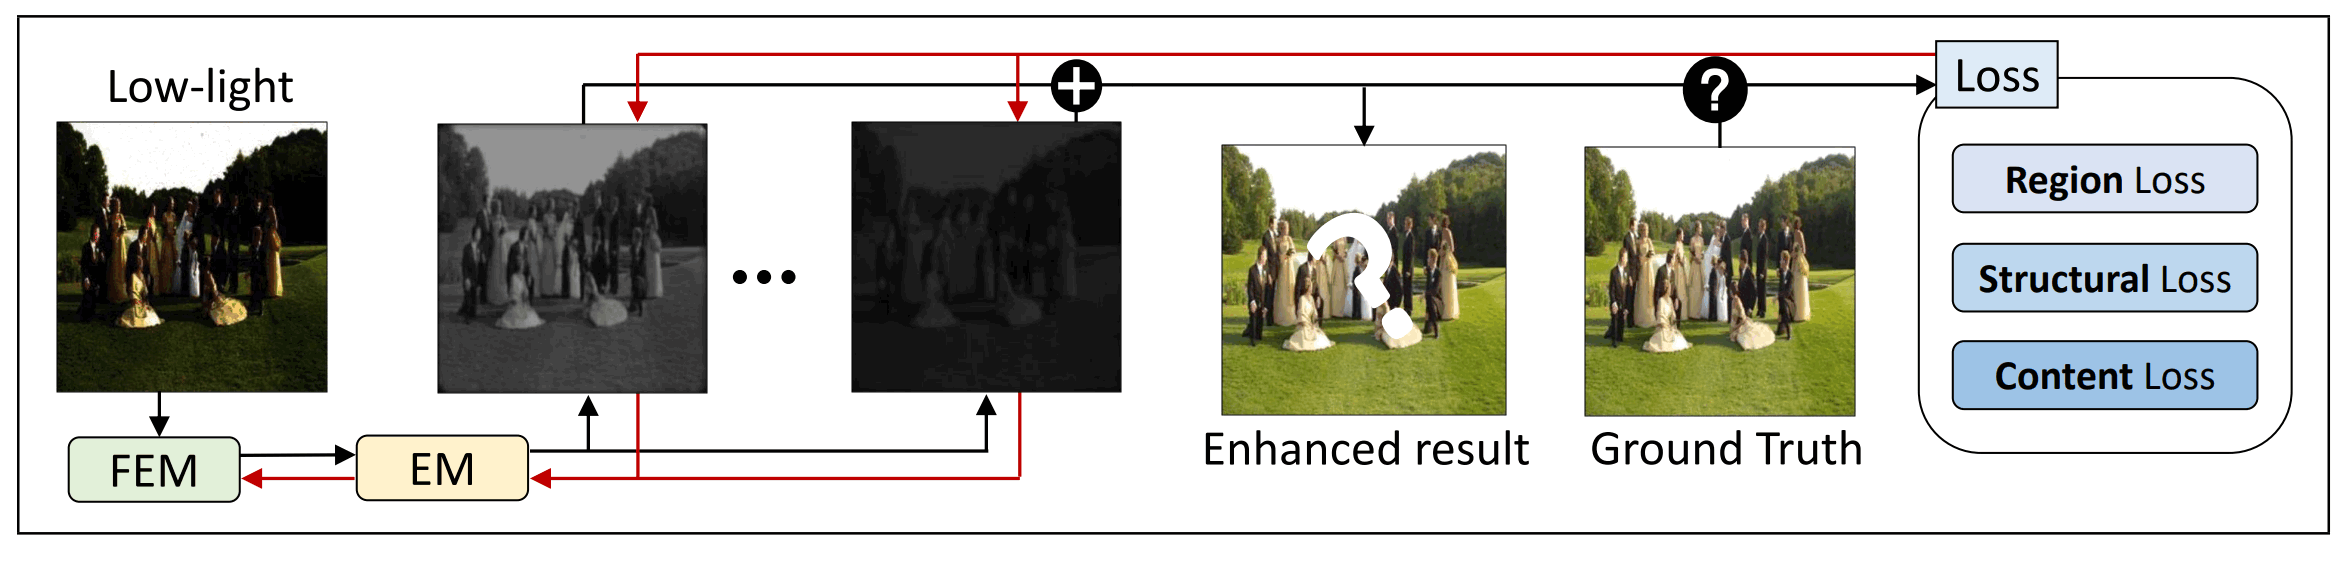
\includegraphics[width=0.8\columnwidth]{proposed_loss_function}
		\captionsetup{font=scriptsize}
		\caption{
			\label{fig: proposed_loss_function} % spaces are big no-no withing labels
			% things like fig: are optional in the label but it helps
			% to orient yourself when you have multiple figures,
			% equations and tables
			Data flow for training. The proposed loss function consists of three parts.
		}
	\end{figure}
	
	\paragraph{Reflectance loss function}
	
	Reflectance loss function是计算机视觉领域中的一种损失函数,常用于图像去雾(image dehazing)任务中。(图像去雾是指通过算法去除图像中由雾霾引起的能见度降低的效果。Reflectance loss function用于衡量生成的去雾图像与真实清晰图像之间的差异,以指导去雾模型的训练过程。)
	
	Reflectance loss function的核心思想是基于图像的反射率(reflectance)属性。反射率是指物体表面对入射光线的反射程度,与雾霾相关的信息主要存在于反射率中。通过计算生成的去雾图像的反射率与真实清晰图像的反射率之间的差异,可以量化生成图像的质量。
	
	具体来说,Reflectance loss function通常使用像素级别的差异度量函数,比如均方误差(Mean Squared Error,MSE)或结构相似性(Structural Similarity,SSIM)等来计算生成图像与真实图像之间的差异。优化过程的目标是最小化Reflectance loss,使得生成的去雾图像能够与真实清晰图像更加接近。
	
	通过引入Reflectance loss作为训练目标,去雾模型可以学习到更准确的雾霾分布和反射率信息,从而生成更清晰的去雾图像。这有助于提高图像去雾算法的性能和质量。
	
	\paragraph{Consistency loss function}
	
	Consistency loss function是一种在机器学习中使用的损失函数,用于提高模型的一致性。它主要用于半监督学习或自监督学习任务中,其中存在一些带有标签的数据(有目标变量的输入-输出对)和一些没有标签的数据(只有输入)。区别于全监督学习,半监督学习针对训练集标记不完整的情况:仅仅部分数据具有标签,然而大量数据是没有标签的。因此,目前半监督学习的关键问题在于如何充分地挖掘没有标签数据的价值。主流的半监督学习方法有下面几种\footnote{https://blog.csdn.net/JYZhang\_CVML/article/details/106817709}:
	
	(1) \textbf{自训练方法(Self-Training)}。这是一种很直观的思路:既然大量数据是没有标签的,那么能否对这些数据生成一些伪标签(Pseuo Labels),对这些伪标签数据的训练从而利用原始的无标签数据。
	
	(2) \textbf{基于对抗学习的方法(Adversarial-Learning-based)}。这类方法基于一种假设,无标签数据(unlabeled data)通常具有和有标签数据(labeled data)在某种程度上类似的潜在标签。所以很自然地,可以采用GAN的图像模拟思路来进行对有标签数据进行类似于无标签数据的数据增强,进而利用无标签数据的潜在知识(latent knowledge)。
	
	(3) \textbf{基于一致性的方法(Consistency-based)}。 这类方法的核心思路在于一致性损失函数Consistency loss function,对于进过扰动的无标签数据,模型应该对其做出一致性的预测——可以理解成一种利用无标签数据进行网络正则化的方法。
	
	一致性损失函数的基本思想是,在模型对相似输入的处理应该具有一致性。它通过对输入进行一些变换或扰动,然后要求模型在这些变换后仍然能够产生相似的输出。如果模型能够在不同的变换下产生一致的输出,那么我们可以认为模型具有一定的鲁棒性和泛化能力。
	
	具体来说,一致性损失函数可以定义为模型在原始输入和变换后输入上的输出之间的差异。常见的一致性损失函数包括均方差损失、平均绝对误差损失、KL散度等。通过最小化一致性损失函数,模型被迫保持对输入的一致性响应,从而提高模型的泛化能力。
	
	需要注意的是,一致性损失函数的具体形式和应用取决于具体的任务和模型架构。它通常与其他损失函数(如分类损失函数或重构损失函数)结合使用,以共同训练模型。
	
	\paragraph{color loss function}
	
	\paragraph{Laplacian loss function}
	
	\subsubsection{细节}
	
	\renewcommand{\tablename}{Table}
	
	% 在LaTeX中,overfull hbox和overfull vbox的警告是由于badness值超过了tolerance值而产生的1。对于每种字体有一个标准的间距,为了使当前行适应宽度,会改变这些间距,如果badness的值超过了tolerance,就会出现overfull或者underfull的警告
	
	\begin{table}[!htbp]
		\centering
		\tiny
		\resizebox{\columnwidth}{!}{ %按照宽度调整调整表格大小
			\begin{tabular}{m{0.01cm}|>{\centering\arraybackslash}m{1.45cm}|>{\centering\arraybackslash}m{1.0cm}|>{\centering\arraybackslash}m{2.6cm}|>{\centering\arraybackslash}m{3.1cm}|>{\centering\arraybackslash}m{3cm}|>{\centering\arraybackslash}m{2.4cm}|>{\centering\arraybackslash}m{2.4cm}|>{\centering\arraybackslash}m{0.9cm}|>{\centering\arraybackslash}m{1.4cm}|>{\centering\arraybackslash}m{1cm}|}
				
				\hline
				
				& \textbf{Method} & \textbf{Learning} & \textbf{Network Structure} & \textbf{Loss Function} & \textbf{Training Data} & \textbf{Testing Data} & \makecell{\textbf{Evaluation Metric}} & \textbf{Format} & \textbf{Platform} & \textbf{Retinex} \\
				
				\hline
				
				\multirowcell{1}{\makecell{\centering \rotatebox{90}{\textbf{2017}}}} & LLNet & SL & SSDA &  SRR loss & simulated by Gamma Correction \& Gaussian Noise & simulated self-selected & PSNR SSIM & RGB & Theano &  \\
				
				\hline
				
				\multirowcell{6}{\makecell{\centering \rotatebox{90}{\textbf{2018}}}} & LightenNet & SL &  four layers & $L_2$ loss & simulated by random illumination values & simulated self-selected & \makecell{PSNR MAE \\ SSIM User Study} & RGB & Caffe MATLAB & \checkmark \\
				
				& Retinex-Net  & SL & multi-scale network & \makecell{$L_1$ loss \\ invariable reflectance loss \\ smoothness loss} & LOL simulated by adjusting histogram & self-selected & - & RGB & TensorFlow & \ \checkmark \\
				
				& MBLLEN & SL & multi-branch fusion & \makecell{SSIM loss \\ perceptual loss \\ region loss} & simulated by Gamma Correction \& Poisson Noise & simulated self-selected & \makecell{PSNR SSIM \\ AB VIF \\ LOE TOMI} & RGB & TensorFlow &  \\
				
				& SCIE & SL & frequency decomposition & \makecell{$L_2$ loss \\ $L_1$ loss \\ SSIM loss} & SCIE & SCIE & PSNR FSIM \qquad Runtime FLOPs & RGB & Caffe MATLAB &  \\
				
				& Chen et al. & SL & U-Net & $L_1$ loss & SID & SID & PSNR SSIM & Raw & TensorFlow &  \\
				
				& Deepexposure & RL & policy network GAN & deterministic policy gradient adversarial loss & MIT-Adobe FiveK & MIT-Adobe FiveK & PSNR SSIM & Raw & TensorFlow &  \\
				
				\hline
				
				\multirowcell{8}{\makecell{\centering \rotatebox{90}{\textbf{2019}\qquad\qquad \qquad\qquad\qquad}}} & Chen et al. & SL & siamese network & \makecell{$L_1$ loss \\ self-consistency loss} & DRV & DRV & \makecell{PSNR SSIM \\ MAE} & Raw & TensorFlow &  \\
				
				
				& Jiang and Zheng & SL & 3D U-Net & \makecell{$L_1$ loss} & SMOID & SMOID & \makecell{PSNR SSIM \\ MSE} & Raw & TensorFlow &  \\
				
				& DeepUPE & SL & illumination map & \makecell{$L_1$ loss \\ smoothness loss \\ color loss} & retouched image pairs & MIT-Adobe FiveK & \makecell{PSNR SSIM \\ User Study} & RGB & TensorFlow & \checkmark \\
				
				& KinD & SL & three subnetworks U-Net & \makecell{reflectance similarity loss \\ illumination smoothness loss \\ mutual consistency loss \\ $L_1$ loss \\ $L_2$ loss \\ SSIM loss \\ texture similarity loss \\ illumination adjustment loss} & LOL & LOL LIME NPE MEF & \makecell{PSNR SSIM \\ LOE NIQE} & RGB & TensorFlow & \checkmark \\
				
				& Wang et al. & SL & two subnetworks pointwise Conv & $L_1$ loss & simulated by camera imaging model & IP100 FNF38 MPI LOL NPE & \makecell{PSNR SSIM \\ NIQE} & RGB & Caffe & \checkmark \\
				
				& Ren et al. & SL & U-Net like network RNN dilated Conv & \makecell{$L_2$ loss \\ perceptual loss \\ adversarial loss} & MIT-Adobe FiveK with Gamma correction \& Gaussion noise & simulated self-selected DPED & PSNR SSIM Runtime & RGB & Caffe &  \\
				
				& EnlightenGAN & UL & U-Net like network & \makecell{adversarial loss \\ self feature preserving loss} & unpaired real images & NPE LIME MEF DICM VV BBD-100K ExDARK & User Study NIQE Classification & RGB & PyTorch &  \\
				
				& ExCNet. & ZSL & fully connected layers & energy minimization loss & real images & $IE_{ps}D$ & \makecell{User Study \\ CDIQA LOD} & RGB & PyTorch &  \\
				
				\hline
				
				\multirowcell{12}{\makecell{\centering \rotatebox{90}{\textbf{2020}\qquad\qquad\qquad\qquad\qquad\qquad\qquad\qquad\qquad\qquad}}} & Zero-DCE & ZSL & U-Net like network & \makecell{spatial consistency loss \\ exposure control loss \\ color constancy loss \\ illumination smoothness loss} & SICE & SICE NPE LIME MEF DICM VV DARK FACE & \makecell{User Study PI \\ PNSR SSIM \\ MAE Runtime \\ Face detection} & RGB & PyTorch & \\
				
				& DRBN & SSL & recursive network & \makecell{SSIM loss \\ perceptual loss \\ adversarial loss} & LOL images selected by MOS & LOL & \makecell{PSNR SSIM \\ SSIM-GC} & RGB & PyTorch & \\
				
				& Lv et al. & SL & U-Net like network & \makecell{Huber loss \\ SSIM loss \\ perceptual loss \\ illumination smoothness loss} & simulated by a retouching module & LOL SICE DeepUPE & \makecell{User Study PSNR \\ SSIM VIF \\ LOE NIQE \\ \#P Runtime \\ Face detection} & RGB & TensorFlow & \checkmark \\
				
				& Fan et al. & SL & four subnetworks U-Net like network feature modulation & \makecell{mutual smoothness loss \\ reconstruction loss \\ illumination smoothness loss \\ cross entropy loss \\ consistency loss \\ SSIM loss \\ gradient loss \\ ratio learning loss} & \makecell{simulated by \\ illumination adjustment,\\ slight color distortion,\\ and noise simulation} & simulated self-selected & \makecell{PSNR SSIM \\ NIQE} & RGB & - & \checkmark \\
				
				& Xu et al. & SL & \makecell{frequency decomposition \\ U-Net like network} & \makecell{$L_2$ loss \\ perceptual loss} & SID in RGB & \makecell{SID in RGB \\ self-selected} & PSNR SSIM & RGB & PyTorch & \\
				
				& EEMEFN & SL & \makecell{U-Net like network \\ edge detection network} & \makecell{$L_1$ loss \\ weighted cross-entropy loss} & SID & SID & PSNR SSIM & Raw & \makecell{TensorFlow \\ PaddlePaddle} & \\
				
				& DLN & SL & residual learning interactive factor back projection network & \makecell{SSIM loss \\ total variation loss} & simulated by illumination adjustment, slight color distortion, and noise simulation & simulated LOL & \makecell{User Study PSNR \\ SSIM NIQE} & RGB & PyTorch & \\
				
				& LPNet & SL & pyramid network & \makecell{$L_1$ loss \\ perceptual loss \\ luminance loss} & \makecell{LOL SID in RGB \\ MIT-Adobe FiveK} & \makecell{LOL SID in RGB \\ MIT-Adobe FiveK \\ MEF NPE DICM VV} & \makecell{PSNR SSIM \\ NIQE \#P \\ FLOPs Runtime} & RGB & PyTorch & \\
				
				& SIDGAN & SL & U-Net & CycleGAN loss & SIDGAN & SIDGAN & PSNR SSIM TPSNR TSSIM ATWE & Raw & TensorFlow & \\
				
				& RRDNet & ZSL & three subnetworks & \makecell{retinex reconstruction loss \\ texture enhancement loss \\ noise estimation loss} & - & \makecell{NPE LIME \\ MEF DICM} & NIQE CPCQI & RGB & PyTorch & \checkmark \\
				
				& TBEFN & SL & \makecell{three stages \\ U-Net like network} & \makecell{SSIM loss \\ perceptual loss \\ smoothness loss}& SCIE LOL & SCIE LOL DICM MEF NPE VV & \makecell{PSNR SSIM \\ NIQE Runtime \\ \#P FLOPs} & RGB & TensorFlow & \checkmark \\ 
				
				& DSLR & SL & \makecell{Laplacian pyramid \\ U-Net like network} & \makecell{$L_2$ loss \\ Laplacian loss \\ color loss} & MIT-Adobe FiveK & MIT-Adobe FiveK self-selected & \makecell{PSNR SSIM \\ NIQMC NIQE \\ BTMQI CaHDC} & RGB & PyTorch & \\
				
				\hline
			\end{tabular}
		}
		\captionsetup{font=scriptsize} %设置标题字体与表格字体一致
		\caption{\label{tab: Summary}
			Summary of essential characteristics of representative deep learning-based methods, including learning strategies, network structures, loss functions, training datasets, testing datasets, evaluation metrics, data formats of input, and whether the models are Retinex-based or not. "simulated" means the testing data are simulated by the same approach as the synthetic training data. "self-selected" stands for the real-world images selected by the authors. "\#P" represents the number of trainable parameters. "-" means this item is not available or not indicated in the paper.} %表格的标题
		
	\end{table}
	
	Table~\ref{tab: Summary}给出了最近几年主流的基于深度学习的LLIE方案,并从不同角度对其进行了划分。
	
	\subsection{Paper reading}
	
	\subsubsection{Switching gaussian mixture variational rnn for anomaly detection of diverse cdn websites}
	
	
	
	\section{个人工作进展}
	
	\subsection{梳理损失函数}
	
	这一周的工作主要是接着梳理上一周未梳理完成的损失函数
	
	1)三个损失函数Consistency loss、Color loss、Laplacian loss
	
	\subsection{复现KinD代码}
	
	KinD\footnote{https://github.com/zhangyhuaee/KinD}采用的是类U-Net网络,且对比使用了多种损失函数,采用的数据集相对较少,且环境配置相对简单,具体见Tab. \ref{tab: Summary}。同时,KinD\cite{10.1145/3343031.3350926}目前引用数量为543,采用的网络架构较为经典,即Retinex-based的思想。
	
		\subsubsection{Requirement}
	
		\begin{python}
		Python
		Tensorflow >= 1.10.0
		numpy, PIL
		\end{python}
	
		\subsubsection{Train}
	
			KinD Network分为三部分(Fig. \ref{fig: network}):(1)图像分解网络:Layer Decomposition Net;(2)反射分量纠正网络:Reflectance Restoration Net;(3)光照分量纠正网络:Illumination Adjustment Net。
	
		\begin{figure}[htbp]
			% read manual to see what [ht] means and for other possible options
			\centering 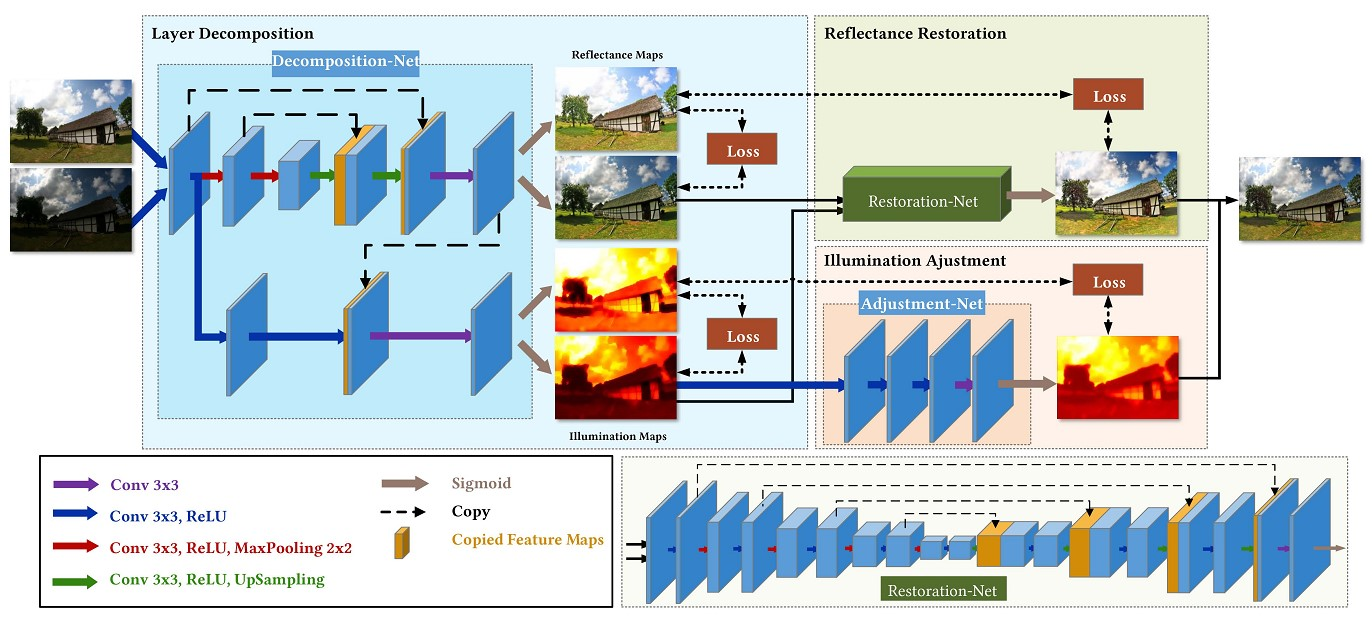
\includegraphics[width=0.8\columnwidth]{network}
			\captionsetup{font=scriptsize}
			\caption{
				\label{fig: network} % spaces are big no-no withing labels
				% things like fig: are optional in the label but it helps
				% to orient yourself when you have multiple figures,
				% equations and tables
				The architecture of our KinD network. Two branches correspond to the reflectance and illumination, respectively. From the perspective of functionality, it also can be divided into three modules, including layer decomposition, reflectance restoration, and illumination adjustment.
			}
		\end{figure}
	
		以暗光/正常光照图像($I_{low}/I_{high}$)对作为训练样本,Layer Decomposition Net对($I_{low}/I_{high}$)依次进行分解,得到光照分量$L_{low}$、$L_{high}$和反射分量$R_{low}$、$R_{high}$。再通过Reflectance Restoration Net和Illumination Adjustment Net得到$\tilde{R}_{low}$和$\tilde{L}_{low}$
	。
	
			\paragraph{Layer Decomposition Net}
		
				Layer Decomposition Net有两个分支,一个分支用于预测反射分量,另一个分支用于预测光照分量,反射分量分支以五层Unet网络为主要网络结构,后接一个卷积层和Sigmoid层。光照分量分支由三个卷积层构成,其中还利用了反射分量分支中的特征图,具体细节可参考论文。
				
				Layer Decomposition Net对($I_l / I_h$)依次进行分解,得到光照分量$L_l$、$L_h$和反射分量$R_l$、$R_h$。
				
				从Fig. \ref{fig: network}可以看出,KinD的损失函数主要由三部分损失构成,它们分别是层分解部分损失、反射重建部分损失以及亮度调整部分损失。
				
				层分解(Layer Decomposition Net)部分损失定义如下:
		
			\begin{equation}
				\mathcal{L}^{LD}=\mathcal{L}_{rec}^{LD}+0.01\mathcal{L}_{rs}^{LD}+0.15\mathcal{L}_{is}^{LD}+0.2\mathcal{L}_{mc}^{LD}
			\end{equation}
			
			其中,$\mathcal{L}_{rs}^{LD}=\left\|R_l-R_h\right\|1$表示反射相似性损失(Reflectance Similarity),即短曝光与长曝光图形的反射图应该是相同的;$$\mathcal{L}_{is}^{LD}=\left\| \frac{\nabla L_{l}}{\max(\left| \nabla I_{l} \right|,\varepsilon)} \right\|_{1} + \left\| {\frac{\nabla L_{h}}{\max (\left| \nabla I_{h} \right| ,\varepsilon)}}\right\|_{1}$$表示亮度平滑损失约束(Illumination Smoothness),它度量了亮度图与输入图像之间的相对结构,边缘区域惩罚较小,平滑区域惩罚较大;$\mathcal{L}_{mc}^{LD}={\left\|M\circ\exp(-c\cdot M)\right \|}_{1}, M=\nabla \mathcal{L}_{l}+\nabla \mathcal{L}_{h}$表示相互一致性约束(Mutual Consistency),它意味着强边缘得以保留,弱边缘被抑制;$\mathcal{L}_{rec}^{LD}={\left \| I_l-R_t \circ \mathcal{L}_l\right\|}_{1} + {\left \| I_h-R_h \circ \mathcal{L}_h\right\|}_{1}$表示重建损失(Reconstruction Error)。
		
			Layer Decomposition Net复现代码如下
			\begin{python}
			# 设置一些训练所需的参数
			batch_size = 10
			patch_size = 48
				
			# 创建一个TensorFlow会话
			sess = tf.Session()
				
			# 定义输入的占位符,这些占位符用于接收低分辨率和高分辨率的输入图像。
			input_low = tf.placeholder(tf.float32, [None, None, None, 3], name='input_low')
			input_high = tf.placeholder(tf.float32, [None, None, None, 3], name='input_high')
				
			# 使用定义的模型构建计算图,DecomNet_simple是一个分解网络模型,它接受输入图像并输出反射和亮度组件
			[R_low, I_low] = DecomNet_simple(input_low)
			[R_high, I_high] = DecomNet_simple(input_high)
				
			# 将反射和亮度组件拼接起来形成输出图像
			# 这一步操作将反射和亮度组件进行通道拼接,以生成输出图像。
			I_low_3 = tf.concat([I_low, I_low, I_low], axis=3)
			I_high_3 = tf.concat([I_high, I_high, I_high], axis=3)
			output_R_low = R_low
			output_R_high = R_high
			output_I_low = I_low_3
			output_I_high = I_high_3
				
			# 定义损失函数
				
			def mutual_i_loss(input_I_low, input_I_high):
			
			# 互信息损失函数的定义
				...
				
			def mutual_i_input_loss(input_I_low, input_im):
			# 输入互信息损失函数的定义
			...
				
			recon_loss_low = tf.reduce_mean(tf.abs(R_low * I_low_3 - input_low))
			recon_loss_high = tf.reduce_mean(tf.abs(R_high * I_high_3 - input_high))
			equal_R_loss = tf.reduce_mean(tf.abs(R_low - R_high))
			i_mutual_loss = mutual_i_loss(I_low, I_high)
			i_input_mutual_loss_high = mutual_i_input_loss(I_high, input_high)
			i_input_mutual_loss_low = mutual_i_input_loss(I_low, input_low)
				
			loss_Decom = 1*recon_loss_high + 1*recon_loss_low + 0.01*equal_R_loss + 0.2*i_mutual_loss + 0.15*i_input_mutual_loss_high + 0.15*i_input_mutual_loss_low
				
			# recon_loss_low 和 recon_loss_high 是重构损失,用于衡量输出图像与输入图像之间的差异。
			# equal_R_loss 是反射一致性损失,用于衡量两个不同尺度下的反射分量之间的一致性。
			# i_mutual_loss 是亮度互信息损失,用于鼓励亮度分量之间的一致性。
			# i_input_mutual_loss_high 和 i_input_mutual_loss_low 是输入亮度与反射之间的互信息损失,用于鼓励输入图像与反射分量之间的一致性。
			\end{python}
			
			最后定义优化器和训练操作
			
			\begin{python}
			# 我们使用 Adam 优化器来最小化损失函数,其中只更新 DecomNet 模型的可训练变量。
			lr = tf.placeholder(tf.float32, name='learning_rate')
			optimizer = tf.train.AdamOptimizer(learning_rate=lr, name='AdamOptimizer')
			var_Decom = [var for var in tf.trainable_variables() if 'DecomNet' in var.name]
			train_op_Decom = optimizer.minimize(loss_Decom, var_list=var_Decom)
			sess.run(tf.global_variables_initializer())
			saver_Decom = tf.train.Saver(var_list=var_Decom)
				
			# 加载数据集
			# 这里使用 glob 函数获取训练集的低分辨率和高分辨率图像的文件名,并进行排序。
			train_low_data = []
			train_high_data = []
			train_low_data_names = glob('./LOLdataset/our485/low/*.png') 
			train_low_data_names.sort()
			train_high_data_names = glob('./LOLdataset/our485/high/*.png') 
			train_high_data_names.sort()
			
			# 定义了一些辅助变量和文件夹路径
			# epoch 表示训练的总轮数,learning_rate 表示学习率,sample_dir 是保存样本图像的文件夹路径,checkpoint_dir 是保存模型检查点的文件夹路径。
			epoch = 2000
			learning_rate = 0.0001
			sample_dir = './Decom_net_train/'
			checkpoint_dir = './checkpoint/decom_net_train/'
			\end{python}
			
				最后开始训练循环
			
			\begin{python}
				for epoch in range(start_epoch, epoch):
				for batch_id in range(start_step, numBatch):
				# 获取一个批次的训练数据
				...
				
				# 执行训练操作,计算损失
				_, loss = sess.run([train_op, train_loss], feed_dict={input_low: batch_input_low, input_high: batch_input_high, lr: learning_rate})
				
				# 打印训练进度和损失
				print("%s Epoch: [%2d] [%4d/%4d] time: %4.4f, loss: %.6f" % (train_phase, epoch + 1, batch_id + 1, numBatch, time.time() - start_time, loss))
				
				# 每隔100个批次保存模型和样本图像
				if (epoch + 1) % 100 == 0:
				print('Saving sample images...')
				sample_results = sess.run([output_R_low, output_R_high, output_I_low, output_I_high], feed_dict={input_low: sample_input_low, input_high: sample_input_high})
				save_images(sample_results, [batch_size, 1], sample_dir + 'train_%d.png' % (epoch + 1))
				
				print('Saving model...')
				saver.save(sess, checkpoint_dir + 'model.ckpt', global_step=epoch + 1)
				
				# 每隔500个批次降低学习率
				if (epoch + 1) % 500 == 0:
				learning_rate /= 10
			\end{python}
			
				在每个 epoch 的训练过程中,当遍历完一个批次后,计算并打印损失值。
				
				当达到一定条件时,例如每隔 100 个批次,保存模型和样本图像。首先,我用当前模型对一部分样本进行推断,并将结果保存为图像文件。然后,保存模型的检查点,以便在需要时恢复模型。
				
				另外,每隔 500 个批次,将学习率除以 10,以实现学习率的衰减。
		
			\paragraph{Reflectance Restoration Net}
			
				作者认为来自低光图像的反射率图比来自明亮光图像的反射率图更容易受到退化的干扰。利用更清晰的反射率作为混乱反射率的参考(非正式的地面实况)。对于寻找Restoration函数,目标简单定义如Eq. \ref{eq: Restoration loss}
				\begin{equation}
					\mathcal{L}^{RR}:={\left\| \hat{R}-R_{h} \right\|}^{2}_{2} - SSIM(\hat{R},R_{h}) + {\left\|\nabla\hat{R}-\nabla R_{h} \right\|}^{2}_{2}
					\label{eq: Restoration loss}
				\end{equation}
				
				Reflectance Restoration Net复现代码如下
				
				\begin{python}
				# 定义一些超参数
				batch_size = 4
				patch_size = 384
					
				# 创建 TensorFlow 会话并配置 GPU 使用
				config = tf.ConfigProto()
				config.gpu_options.allow_growth = True
				sess=tf.Session(config=config)
					
				# 定义输入占位符
				input_decom = tf.placeholder(tf.float32, [None, None, None, 3], name='input_decom')
				input_low_r = tf.placeholder(tf.float32, [None, None, None, 3], name='input_low_r')
				input_low_i = tf.placeholder(tf.float32, [None, None, None, 1], name='input_low_i')
				input_high_r = tf.placeholder(tf.float32, [None, None, None, 3], name='input_high_r')
					
				# 构建模型的图结构
				[R_decom, I_decom] = DecomNet_simple(input_decom)
				decom_output_R = R_decom
				decom_output_I = I_decom
				output_r = Restoration_net(input_low_r, input_low_i)
				\end{python}
				
				loss\_restoration = loss\_square + loss\_ssim + loss\_grad:这一行代码定义了总的损失函数 loss\_restoration,它是由三个部分的损失函数相加而成。loss\_square 是图像修复前后像素差的平方和的均值,用来衡量修复后图像与原始图像的像素差异。loss\_ssim 是结构相似性损失,用来衡量修复后图像与原始图像的结构相似性。loss\_grad 是梯度损失,用来衡量修复后图像与原始图像的梯度差异。通过将这三个损失函数相加,可以综合考虑图像修复的像素准确性、结构相似性和梯度一致性。
				
				\begin{python}
				# 定义损失函数
				def grad_loss(input_r_low, input_r_high):
					input_r_low_gray = tf.image.rgb_to_grayscale(input_r_low)
					input_r_high_gray = tf.image.rgb_to_grayscale(input_r_high)
					x_loss = tf.square(gradient(input_r_low_gray, 'x') - gradient(input_r_high_gray, 'x'))
					y_loss = tf.square(gradient(input_r_low_gray, 'y') - gradient(input_r_high_gray, 'y'))
					grad_loss_all = tf.reduce_mean(x_loss + y_loss)
					return grad_loss_all
					
				def ssim_loss(output_r, input_high_r):
					output_r_1 = output_r[:,:,:,0:1]
					input_high_r_1 = input_high_r[:,:,:,0:1]
					ssim_r_1 = tf_ssim(output_r_1, input_high_r_1)
					output_r_2 = output_r[:,:,:,1:2]
					input_high_r_2 = input_high_r[:,:,:,1:2]						ssim_r_2 = tf_ssim(output_r_2, input_high_r_2)
					output_r_3 = output_r[:,:,:,2:3]
					input_high_r_3 = input_high_r[:,:,:,2:3]
					ssim_r_3 = tf_ssim(output_r_3, input_high_r_3)
					ssim_r = (ssim_r_1 + ssim_r_2 + ssim_r_3)/3.0
					loss_ssim1 = 1-ssim_r
					return loss_ssim1
					
				loss_square = tf.reduce_mean(tf.square(output_r  - input_high_r))
				loss_ssim = ssim_loss(output_r, input_high_r)			
				loss_grad = grad_loss(output_r, input_high_r)
				loss_restoration = loss_square + loss_grad + loss_ssim
				\end{python}

				lr = tf.placeholder(tf.float32, name='learning\_rate'):这一行代码创建了一个占位符lr,用于传入学习率。占位符是在TensorFlow中用于表示在运行时提供数据的节点。在训练过程中,可以通过向lr传递不同的学习率值来控制模型的学习速度。
				
				\begin{python}
				# 定义优化器和训练操作
				lr = tf.placeholder(tf.float32, name='learning_rate')
				optimizer = tf.train.AdamOptimizer(lr)
				train_op = optimizer.minimize(loss_restoration)
				
				# 初始化变量并创建模型保存器
				sess.run(tf.global_variables_initializer())
				saver=tf.train.Saver(max_to_keep=50)
					
				# 定义一些训练过程中需要使用的函数和变量
				train_dataset = glob('./data/train/*')
				steps_per_epoch = len(train_dataset) // batch_size
				global_step = 0
				learning_rate = 0.0001
				\end{python}
				
				最后开始训练循环,for epoch in range(20): 这个循环用于控制训练的迭代次数,每个迭代称为一个 epoch。在每个 epoch 中,数据集被随机打乱,以增加数据的随机性。这样,整个训练过程会逐步优化模型参数,以达到更好的图像修复效果。
				
				第2行代码使用 random.shuffle 函数随机打乱训练数据集的顺序,以增加数据的随机性。
				
				第3行使用嵌套循环用于遍历每epoch 中的小批量数据。steps\_per\_epoch 是每个 epoch 中的步骤数量,通过将训练数据集的大小除以批量大小得到。
				
				第5行代码调用了 load\_data 函数,从训练数据集中加载一批数据。train\_dataset[] 表示取出当前批次的训练数据,patch\_size 是图像块的大小。

				第7行代码通过调用 sess.run 函数执行了一次训练操作和损失函数的计算,并将结果赋值给变量 loss\_value、loss\_square\_value、loss\_ssim\_value 和 loss\_grad\_value。
				
				\begin{python}
				for epoch in range(20):
					random.shuffle(train_dataset)
				for batch_id in range(steps_per_epoch):
					start_time = time.time()					
					input_low_r_data, input_low_i_data, input_high_r_data = load_data(train_dataset[batch_id*batch_size:(batch_id+1)*batch_size], patch_size)
					
					_, loss_value, loss_square_value, loss_ssim_value, loss_grad_value = sess.run([train_op, loss_restoration, loss_square, loss_ssim, loss_grad], feed_dict={input_low_r: input_low_r_data, input_low_i: input_low_i_data, input_high_r: input_high_r_data, lr: learning_rate})
					
					duration = time.time() - start_time
					
					global_step += 1
					
					if batch_id % 100 == 0:
						print('Epoch {:d}/{:d} Batch {:d}/{:d} loss = {:.6f}, loss_square = {:.6f}, loss_ssim = {:.6f}, loss_grad = {:.6f}, time = {:.2f}s'.format(epoch + 1, 20, batch_id + 1, steps_per_epoch, loss_value, loss_square_value, loss_ssim_value, loss_grad_value, duration))
				\end{python}
				
				通过这段代码不难看出,其实现了一个图像训练模型的过程,包括了数据预处理、模型构建、损失函数定义、优化器设置以及训练过程的迭代。它使用了 TensorFlow 框架和一些自定义的模块和函数来完成图像修复任务的训练。
				
				
			\paragraph{Illumination Adjustment Net}
		
				由于不存在用于图像的地面实况光照级别。因此,为了满足不同的需求,需要一种机制来灵活地将一种光照条件转换为另一种光照条件。数据集中是成对的照明图。虽然不知道之间的确切关系,但是可以大致计算强度的元素级比率$\alpha(L_t / L_s)$。这个比例可以作为指标来训练一个调整函数从一个光照条件$L_s$到另一个标准$L_t$,如果调整光照的水平更高,则$\alpha>1$,否则$\alpha \le 1$。在测试阶段,$\alpha$可以由用户指定。该网络是轻量级的,包含3个conv层(2个conv+ReLu和1个conv)和1个Sigmoid层。我们注意到指标$\alpha$是作为输入的一部分扩展到一个特性映射上。(代码中是把这个比值扩展成一个常数通道与输入图像合并变成4通道)。光照分量的纠正与反射分量纠正类似,这里同样使用高光照图光照分量$L_t$,作为真值约束训练,网络预测得到的纠正后反射分量为$\tilde{L}$,等式Eq. \ref{Illumination Adjustment loss}是照明调节网的损失函数\footnote{https://blog.csdn.net/xspyzm/article/details/106162581}。
				\begin{equation}
					\mathcal{L}^{IA}:={\left\| \hat{L}-L_{t} \right\|}^{2}_{2} + {\left\| \left|\nabla\hat{L}\right|-\nabla L_{t} \right\|}^{2}_{2}
					\label{Illumination Adjustment loss}
				\end{equation}
			
			\begin{python}
			# 设置一些训练相关的参数
			batch_size = 10
			patch_size = 48
			
			# 创建TensorFlow会话
			sess = tf.Session()
			
			# 定义输入占位符
			input_decom = tf.placeholder(tf.float32, [None, None, None, 3], name='input_decom')
			input_low_i = tf.placeholder(tf.float32, [None, None, None, 1], name='input_low_i')
			input_low_i_ratio = tf.placeholder(tf.float32, [None, None, None, 1], name='input_low_i_ratio')
			input_high_i = tf.placeholder(tf.float32, [None, None, None, 1], name='input_high_i')
			\end{python}
		
			下面的代码构建了图像处理的模型。首先通过DecomNet\_simple函数构建了一个分解网络模型,将输入的图像分解为反射分量和光照分量,分别保存在decom\_output\_R和decom\_output\_I中。然后通过Illumination\_adjust\_net函数构建了一个光照调整网络模型,用于调整输入的光照分量,保存在output\_i中。
			
			\begin{python}
			# 构建模型
			[R_decom, I_decom] = DecomNet_simple(input_decom)
			decom_output_R = R_decom
			decom_output_I = I_decom
			output_i = Illumination_adjust_net(input_low_i, input_low_i_ratio)
			\end{python}
			
			下列的代码定义了损失函数。grad\_loss函数计算输入的两个图像的梯度差异,并计算梯度差异的平均值。loss\_grad表示光照分量的梯度损失,loss\_square表示光照分量的均方差损失,而loss\_adjust是将梯度损失和均方差损失相加得到的总体损失。
			
			\begin{python}
			# 定义损失函数
			def grad_loss(input_i_low, input_i_high):
				x_loss = tf.square(gradient(input_i_low, 'x') - gradient(input_i_high, 'x'))
				y_loss = tf.square(gradient(input_i_low, 'y') - gradient(input_i_high, 'y'))
				grad_loss_all = tf.reduce_mean(x_loss + y_loss)
				return grad_loss_all
			
			loss_grad = grad_loss(output_i, input_high_i)
			loss_square = tf.reduce_mean(tf.square(output_i  - input_high_i))
			loss_adjust =  loss_square + loss_grad
			\end{python}
			
			这些代码定义了一个Adam优化器,并使用它最小化总体损失loss\_adjust。train\_vars表示可训练的变量,这些变量将会在训练过程中更新。
			
			\begin{python}
			# 定义优化器和训练操作
			train_vars = tf.trainable_variables()
			train_op_adjust = tf.train.AdamOptimizer(learning_rate=0.0001).minimize(loss_adjust, var_list=train_vars)
			\end{python}
			
			这行代码使用glob函数加载训练数据的文件路径。'./data/train/*.png'表示加载./data/train/路径下所有以.png结尾的文件。
			
			\begin{python}
			# 初始化变量
			sess.run(tf.global_variables_initializer())
			
			# 加载训练数据
			train_data = glob('./data/train/*.png')
			\end{python}
		
			这段代码中的循环用于进行训练。外层循环是30个训练轮次(epochs),内层循环根据批大小将训练数据分成小批次进行训练。首先通过get\_image函数加载批次的图像文件,并将它们转换为浮点数类型的数组。然后将图像数组归一化到[0, 1]的范围。接下来,将归一化后的低光照图像和差值图像分别作为输入的低光照图像和高光照图像。将它们扩展维度,以匹配占位符的形状。然后执行训练操作train\_op\_adjust,并获取损失函数的值。
		
			\begin{python}
			# 开始训练过程
			for ep in range(30):
				for idx in range(len(train_data)//batch_size):
					batch_files = train_data[idx*batch_size:(idx+1)*batch_size]
					batch = [get_image(batch_file) for batch_file in batch_files]
					batch_images = np.array(batch).astype(np.float32)
					batch_low_images = batch_images / 255.0
					batch_high_images = batch_images - batch_low_images
					batch_low_images = np.expand_dims(batch_low_images[:,:,:,0], axis=3)
					batch_high_images = np.expand_dims(batch_high_images[:,:,:,0], axis=3)
					batch_low_images_ratio = np.expand_dims(batch_low_images[:,:,:,0]/255.0, axis=3)
					_, loss_adjust_value, loss_grad_value, loss_square_value = sess.run([train_op_adjust, loss_adjust, loss_grad, loss_square], feed_dict={input_decom: batch_images, input_low_i: batch_low_images, input_low_i_ratio: batch_low_images_ratio, input_high_i: batch_high_images})
					
			# 打印训练过程中的损失值,`\%2d`表示打印整数,占用两位字符的宽度;`\%.4f`表示打印浮点数,保留四位小数		
			print("Epoch: [%2d], step: [%2d], loss_adjust: [%.4f], loss_grad: [%.4f],loss_square: [%.4f]" % (ep+1, idx+1, loss_adjust_value, loss_grad_value, loss_square_value))
			
			# 保存模型
			saver.save(sess, "./model/model.ckpt")
			\end{python}
			
		\paragraph{Evaluation}
		
		%		\begin{python}
			
			
			%		\end{python}
	
	
	\section{下周工作计划}
	
	(1) 继续复现并详细分析KinD的项目代码,目前架构中的三个结构(Fig. \ref{fig: network})完成其中的训练和代码分析,因此,下周工作计划是尝试去评估模型,其中的model.py还没仔细去看,只是把训练的过程实施了一遍。
	
	(2) 继续整理各类损失函数的区别。按照Table\ref{tab: Summary}中整理的不同文献所采用的损失函数,弄清楚各类损失函数的作用。
	
	(3) 试着更加在说明代码的时候让文档更加规范化,感觉目前的格式有些随意。
	
	(4) 本周删去了关于“华为杯”的思考,这一章节,下一周关于第二个挑战可能会按照Paper\cite{9796836}更多的提出自己的思考。
	
	
	%	\section{Analysis}
	
	%	In this section you will need to show your experimental results. Use tables and
	%	graphs when it is possible. Table~\ref{tbl:bins} is an example.
	
	%	\begin{table}[ht]
		%		\begin{center}
			%			\caption{Every table needs a caption.}
			%			\label{tbl:bins} % spaces are big no-no withing labels
			%			\begin{tabular}{|ccc|} 
				%				\hline
				%				\multicolumn{1}{|c}{$x$ (m)} & \multicolumn{1}{c|}{$V$ (V)} & \multicolumn{1}{c|}{$V$ (V)} \\
				%				\hline
				%				0.0044151 &   0.0030871 &   0.0030871\\
				%				0.0021633 &   0.0021343 &   0.0030871\\
				%				0.0003600 &   0.0018642 &   0.0030871\\
				%				0.0023831 &   0.0013287 &   0.0030871\\
				%				\hline
				%			\end{tabular}
			%		\end{center}
		%	\end{table}
	%	
	%	Analysis of equation~\ref{eq:aperp} shows ...
	%	
	%	Note: this section can be integrated with the previous one as long as you
	%	address the issue. Here explain how you determine uncertainties for different
	%	measured values. Suppose that in the experiment you make a series of
	%	measurements of a resistance of the wire $R$ for different applied voltages
	%	$V$, then you calculate the temperature from the resistance using a known
	%	equation and make a plot  temperature vs. voltage squared. Again suppose that
	%	this dependence is expected to be linear~\cite{Cyr}, and the proportionality coefficient
	%	is extracted from the graph. Then what you need to explain is that for the
	%	resistance and the voltage the uncertainties are instrumental (since each
	%	measurements in done only once), and they are $\dots$. Then give an equation
	%	for calculating the uncertainty of the temperature from the resistance
	%	uncertainty. Finally explain how the uncertainty of the slop of the graph was
	%	found (computer fitting, graphical method, \emph{etc}.)
	%	
	%	If in the process of data analysis you found any noticeable systematic
	%	error(s), you have to explain them in this section of the report.
	%	
	%	It is also recommended to plot the data graphically to efficiently illustrate
	%	any points of discussion. For example, it is easy to conclude that the
	%	experiment and theory match each other rather well if you look at
	%	Fig.~\ref{fig:samplesetup} and Fig.~\ref{fig:exp_plots}.
	%	
	%	\begin{figure}[ht] 
		%		\centering
		%		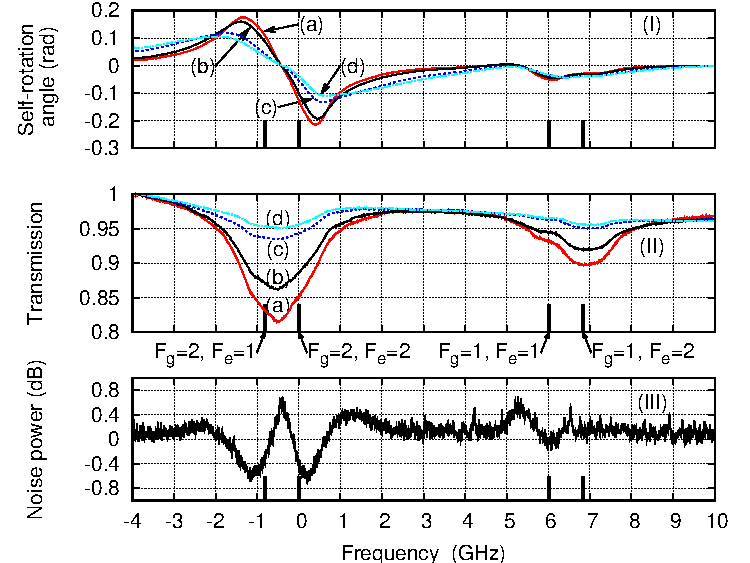
\includegraphics[width=0.5\columnwidth]{sr_squeezing_vs_detuning}
		%		
		%		% some figures do not need to be too wide
		%		\caption{
			%			\label{fig:exp_plots}  
			%			Every plot must have axes labeled.
			%		}
		%	\end{figure}
	
	
	%	\section{Conclusions}
	%	Here you briefly summarize your findings.
	
	%++++++++++++++++++++++++++++++++++++++++
	% References section will be created automatically 
	% with inclusion of "thebibliography" environment
	% as it shown below. See text starting with line
	% \begin{thebibliography}{99}
		% Note: with this approach it is YOUR responsibility to put them in order
		% of appearance.
		
		\renewcommand{\refname}{References}
		
		
		%	\begin{thebibliography}{00}
			
			%		\bibitem{b1}\label{cite:b1}
			%		W. Wang, C. Wei, W. Yang and J. Liu, "GLADNet: Low-Light Enhancement Network with Global Awareness," 2018 13th IEEE International Conference on Automatic Face \& Gesture Recognition (FG 2018), Xi'an, China, 2018, pp. 751-755, DOI: 10.1109/FG.2018.00118.
			
			%		\bibitem{b2}\label{cite:b2}
			%		A.\ Mahajan, K.\ Somaraj and M. Sameer, "Adopting Artificial Intelligence Powered ConvNet To Detect Epileptic Seizures," 2020 IEEE-EMBS Conference on Biomedical Engineering and Sciences (IECBES), Langkawi Island, Malaysia, 2021, pp. 427-432, DOI: 10.1109/IECBES48179.2021.9398832.
			
			%		\bibitem{Cyr}
			%		N.\ Cyr, M.\ T$\hat{e}$tu, and M.\ Breton,
			% "All-optical microwave frequency standard: a proposal,"
			%		IEEE Trans.\ Instrum.\ Meas.\ \textbf{42}, 640 (1993).
			
			
			
			%	\end{thebibliography}
		
		\bibliographystyle{unsrt}
		\bibliography{reference}
		
		
	\end{document}
